\documentclass[final,a4paper,openany,12pt]{mwbk}
%\documentclass[final,a4paper,openright,12pt]{mwbk} % każdy rozdział zaczyna się na stronie nieparzystej
\usepackage{polski}
\usepackage[utf8]{inputenc}
\usepackage{fancyhdr}
\usepackage{url}
\usepackage{algorithm}
\usepackage{algpseudocode}
\usepackage{enumerate}
\usepackage{subcaption}
\captionsetup{compatibility=false}
\usepackage{titlesec}
\usepackage{amsmath}
\usepackage{listings}
\lstset{
language=Python,
breaklines=true,
tabsize=2,
breaklines  = true,
breakatwhitespace   = false,
prebreak= \space,
postbreak   = \space  
}   



\titleformat{\section}[runin]
{\normalfont\Large\bfseries}{\thesection}{1em}{}
\titleformat{\subsection}[runin]
{\normalfont\large\bfseries}{\thesubsection}{1em}{}




\usepackage{makeidx}  % allows index generation
\usepackage{graphicx} % standard LaTeX graphics tool
                      % for including eps-figure files
\graphicspath{{img/}{img/Zegarek}}
\usepackage{float}


%\prefixing %polskie znaki: /a /c /e /z /x /o /s /l /A /C itd. %ZAKOMENTOWANE BO SIE NIE DA UZYWAC "/"

\renewcommand*\listalgorithmname{Spis algorytmów\protect} % łatka na niedoróbkę w spisie algorytmów - nie usuwać!

% zestaw przydatny, kiedy trzeba regulować szerokość kolumn w tablicy:
%%\usepackage{longtable}
%\usepackage{array}
%\newcolumntype{L}[1]{>{\raggedright\let\newline\\\arraybackslash\hspace{0pt}}m{#1}}
%\newcolumntype{C}[1]{>{\centering\let\newline\\\arraybackslash\hspace{0pt}}m{#1}}
%\newcolumntype{R}[1]{>{\raggedleft\let\newline\\\arraybackslash\hspace{0pt}}m{#1}}

\newtheorem{twr}{Twierdzenie}[section]

% ustawienia do wydruku dwustronnego z uwzględnieniem dodatkowego miejsca na zszycie
\setlength{\oddsidemargin}{0.46cm}   %margines nieparzysty
\setlength{\evensidemargin}{-0.54cm} %margines parzysty
\setlength{\textwidth}{16cm}         %szerokość tekstu na stronie
\linespread{1.1}    % lekkie zwiększenie odstępu między liniami, żeby tekst nie był taki ścisły, ponieważ
                    % Odstęp pojedynczej interlinii nie jest komfortowy, kiedy trzeba czytać strony A4
% koniec ustawień

%\makeindex            % used for the subject index
                      % please use the style sprmidx.sty with
                      % your makeindex program
\begin{document}

\begin{titlepage}
\vspace{-0.5cm}

{\centering
{\footnotesize
\begin{tabular}{c}
UNIWERSYTET KARDYNAŁA STEFANA WYSZYŃSKIEGO\\
W WARSZAWIE\\
\end{tabular}
}
\vspace{2.5cm}

{\footnotesize
\begin{tabular}{c}
WYDZIAŁ MATEMATYCZNO-PRZYRODNICZY\\
SZKOŁA NAUK ŚCISŁYCH\\
\end{tabular}
}
\vspace{2.5cm}

\renewcommand{\arraystretch}{1.5} % zwiększamy odległość między wierszami

{\normalsize
\begin{tabular}{c}
Katarzyna Mitrus\\
Michał Słotwiński\\
\end{tabular}
}

\vspace{1.5cm}

{\large
\begin{tabular}{c}

Wprowadzenie do Przetwarzania Obrazów\\
Sprawozdanie z laboratorium\\

\end{tabular}
}

}

\renewcommand{\arraystretch}{1} % przywracamy domyślną odległość miedzy wierszami

\vspace{5cm}

\hspace{6cm}
\begin{tabular}{l}
Prowadzący:\\
prof. Wojciech Mokrzycki\\

\end{tabular}

\vspace{4cm}

{\centering

{\small
\begin{tabular}{c}
{Warszawa, 2018}\\
\end{tabular}
}

}
\end{titlepage}

\tableofcontents
\listoffigures
%\listoftables
%\listofalgorithms

\sloppy


\chapter {Wstęp}

Laboratoria oh oh...~\cite{BookMok} %przynajmniej jedna cytacja dla kompilatora LATEX


\section {Specyfikacja wykorzystanego fortmatu obrazu}

\section {Intstrukcja obsługi programu}



\chapter{Operacje ujednolicania obrazów}
1. ujednolicenie obrazów szarych geometryczne (liczba wierszy i kolumn piksli)
2. ujednolicenie obrazów szarych rozdzielczościowe (w rastrze)
3. ujednolicenie obrazów RGB geometryczne (liczba wierszy i kolumn piksli)
4. ujednolicenie obrazów RGB rozdzielczościowe (w rastrze)

\chapter{Operacje sumowania arytmetycznego obrazów szarych}

Arytmetyczne operacje między pikslami $p$ i $q$ dwóch obrazów są używane w wielu działach przetwarzania obrazów. Przeprowadzane się je wykonując działania na pojedynczych pikslach i są uwarunkowane wymaganiami zależnymi od typu operacji. 
Po operacjach arytmetycznych zwykle niezbędna jest normalizacja. W przedstawionych zadaniach do normalizacji wykorzystano wzór:
	
	\begin{center}
		$ f_{norm} = Z_{rep}[(f - f_{min}) / (f_{max} - f_{min})] $
	\end{center}

\section {Sumowanie (określonej) stałej z obrazem}
%\subsection*{Opis algorytmu}
\hfill
\\\\
\indent
Algorytm sumowania obrazu szarego z określoną stałą polega na dodaniu do każdej wartości pojedynczego piksla stałej liczby.
Po operacji sumowania następuje normalizacja obrazu.

	\begin{enumerate}	
		\item Policz sumy wartości kazdego piksla ze stałą ($const$).
		\item Jeżeli jedna z tych sum jest większa niż 255 to:
		\item Wybierz największą sumę  $Q_{max}$ i policz $D_{max}$ ze wzoru: $D_{max}[i,j] = (Q_{max}[i,j] - 255)$ 
		\item Oblicz $X = D_{max} / 255$
		\item Policz sumy ze wzoru
		\begin{center}$Q[i,j] = P[i,j] - (P[i,j]* X) + const - (const * X) $ \\

		\end{center}
	\end{enumerate}

\begin{figure}[H]
	\begin{center}
		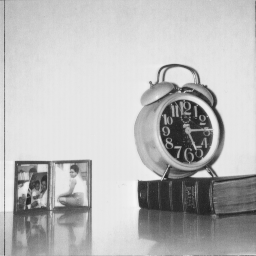
\includegraphics[width=0.3\textwidth]{1/1Gray_Const_Sum_Original}
		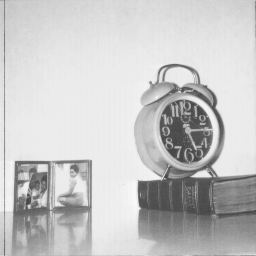
\includegraphics[width=0.3\textwidth]{1/1Gray_Const_Sum_Result}
		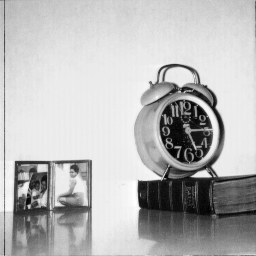
\includegraphics[width=0.3\textwidth]{1/1Gray_Const_Sum_Result_Norm}
	\end{center}
	\caption{(Od lewej) Szary obraz wejściowy, obraz po sumowaniu ze stałą = 50, obraz po normalizacji }
\end{figure}

\begin{figure}[H]
	\begin{center}
		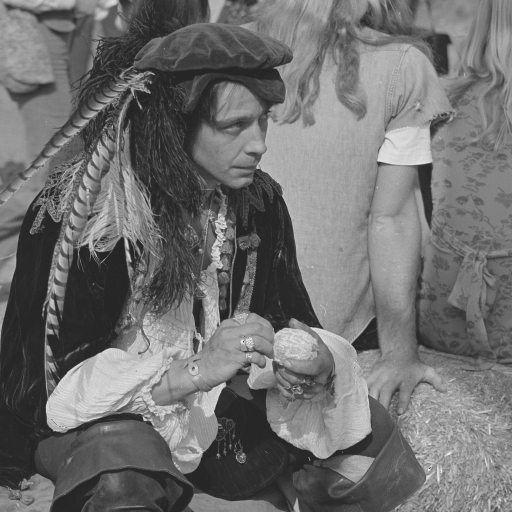
\includegraphics[width=0.3\textwidth]{2/2Gray_Const_Sum_Original}
		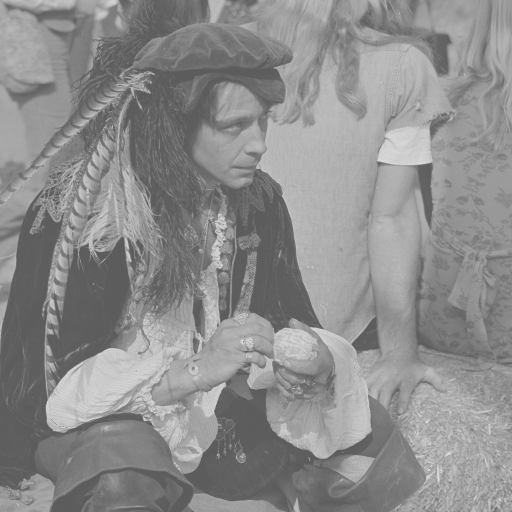
\includegraphics[width=0.3\textwidth]{2/2Gray_Const_Sum_Result}
		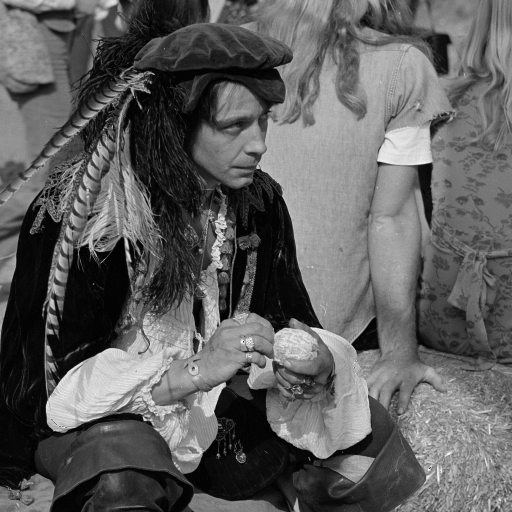
\includegraphics[width=0.3\textwidth]{2/2Gray_Const_Sum_Result_Norm}
	\end{center}
	\caption{(Od lewej) Szary obraz wejściowy, obraz po sumowaniu ze stałą = 100, obraz po normalizacji }
\end{figure}

\subsection*{Kod źródłowy}

\begin{lstlisting}[caption=Sumowanie obrazu szarego ze stałą]

image_matrix = self.im1
width = image_matrix.shape[1]    # szereoksc
height = image_matrix.shape[0]   # wysokosc

result_matrix = np.zeros((width, height), dtype=np.uint8)

# Inicjalizacja zmiennych
Q_max = 0
D_max = 0
X = 0
f_min = 255
f_max = 0

for y in range(height):
    for x in range(width):  
        # Obliczanie sumy
        L = int(image_matrix[x][y]) + int(const)

        # Poszukiwanie maksimum
        if Q_max < L:
            Q_max = L

# Sprawdzenie czy przekracza zakres
if Q_max > 255:
    D_max = Q_max - 255
    X = (D_max/255)

# Obliczenie sumy z uwzglednieniem zakresu
for y in range(height):
    for x in range(width): 
        L = (image_matrix[x][y] - (image_matrix[x][y] * X)) + (const - (const * X))

        # Zaokroglenie do najblizszej wartosci calkowitej z gory
        # i przypisanie wartosci
        result_matrix[x][y] = math.ceil(L)

        # Poszukiwanie minimum i maksimum
        if f_min > L:
            f_min = L
        if f_max < L:
            f_max = L

# Normalizacja
norm_matrix = np.zeros((width, height), dtype=np.uint8)
for y in range(height):
    for x in range(width):
        norm_matrix[x][y] = 255 * ((result_matrix[x][y] - f_min) / (f_max - f_min))

\end{lstlisting}



\section {Sumowanie dwóch obrazów}
\hfill
\\\\
\indent

\begin{figure}[H]
	\begin{center}
		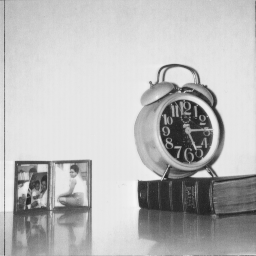
\includegraphics[width=0.3\textwidth]{1/1Gray_Img1_Sum_Original}
		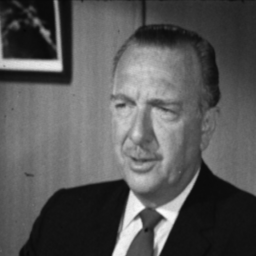
\includegraphics[width=0.3\textwidth]{1/1Gray_Img2_Sum_Original}
		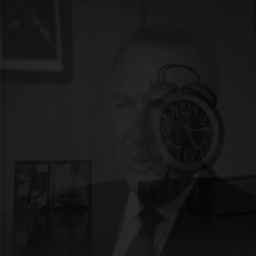
\includegraphics[width=0.3\textwidth]{1/1Gray_Img_Sum_Result}
		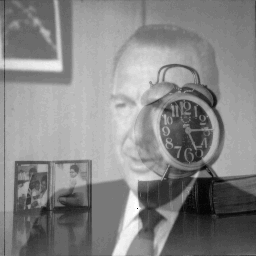
\includegraphics[width=0.3\textwidth]{1/1Gray_Img_Sum_Result_Norm}
	\end{center}
	\caption{(Od lewej) Pierwsze dwa to szare obrazy wejściowe, następnie obraz powstały w wyniku sumowania obrazów, poniżej obraz wynikowy po normalizacji }
\end{figure}

\begin{figure}[H]
	\begin{center}
		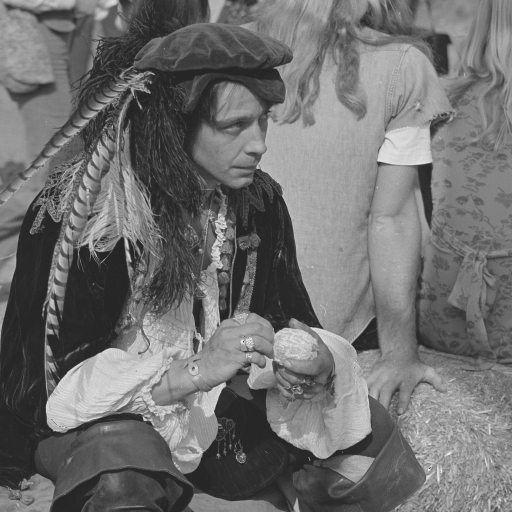
\includegraphics[width=0.3\textwidth]{2/2Gray_Img1_Sum_Original}
		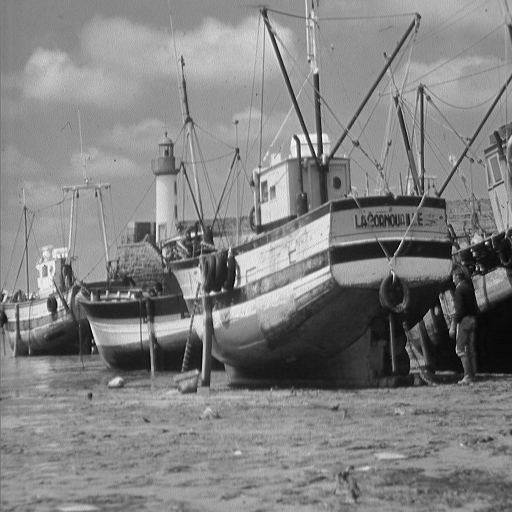
\includegraphics[width=0.3\textwidth]{2/2Gray_Img2_Sum_Original}
		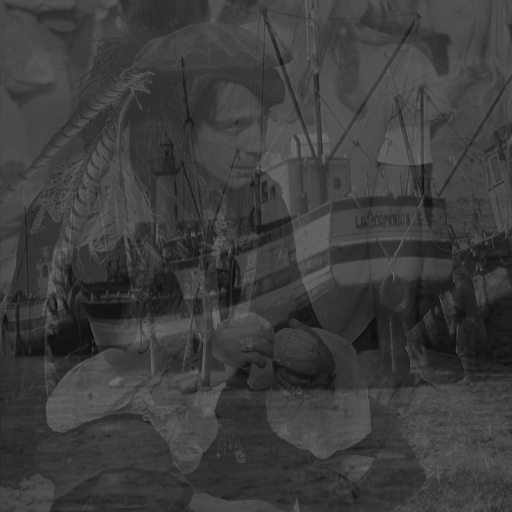
\includegraphics[width=0.3\textwidth]{2/2Gray_Img_Sum_Result}
		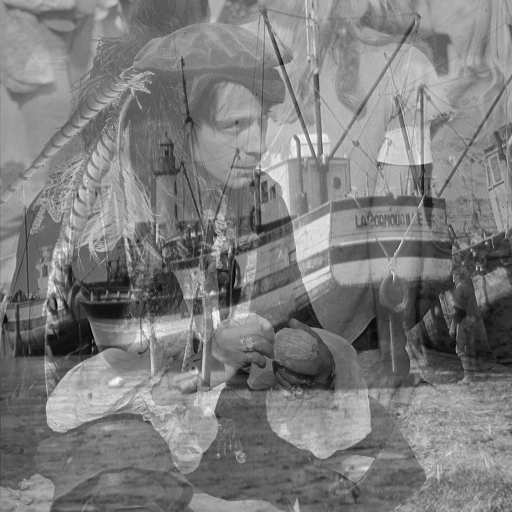
\includegraphics[width=0.3\textwidth]{2/2Gray_Img_Sum_Result_Norm}
	\end{center}
	\caption{(Od lewej) Pierwsze dwa to szare obrazy wejściowe, następnie obraz powstały w wyniku sumowania obrazów, poniżej obraz wynikowy po normalizacji }
\end{figure}


\begin{lstlisting}[caption=Sumowanie obrazów szarych]

image1_matrix = self.im1
image2_matrix = self.im2
height = image1_matrix.shape[0]   # wysokosc
width = image1_matrix.shape[1]    # szereoksc

result_matrix = np.zeros((width, height), dtype=np.uint8)

# Inicjalizacja zmiennych
Q_max = 0
D_max = 0
X = 0
f_min = 255
f_max = 0

for y in range(height):
    for x in range(width):  

        # Obliczanie sumy
        L = int(image1_matrix[x][y]) + int(image2_matrix[x][y])

        # Poszukiwanie maksimum
        if Q_max < L:
            Q_max = L

# Sprawdzenie czy przekracza zakres
if Q_max > 255:
    D_max = Q_max - 255
    X = (D_max/255)

# Obliczenie sumy z uwzglednieniem zakresu
for y in range(height):
    for x in range(width): 
        L = (image1_matrix[x][y] - (image1_matrix[x][y] * X)) + (image2_matrix[x][y] - (image2_matrix[x][y] * X))

        # Zaokroglenie do najblizszej wartosci calkowitej z gory
        # i przypisanie wartosci
        result_matrix[x][y] = math.ceil(L)
        
        # Poszukiwanie minimum i maksimum
        if f_min > L:
            f_min = L
        if f_max < L:
            f_max = L

# Normalizacja
norm_matrix = np.zeros((width, height), dtype=np.uint8)
for y in range(height):
    for x in range(width):
        norm_matrix[x][y] = 255 * ((result_matrix[x][y] - f_min) / (f_max - f_min))

\end{lstlisting}

\section {Mnożenie obrazu przez zadaną liczbę}
\hfill
\\\\
\indent

\begin{figure}[H]
	\begin{center}
		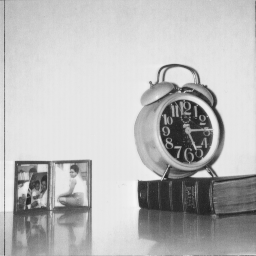
\includegraphics[width=0.3\textwidth]{1/1Gray_Const_Multipl_Original}
		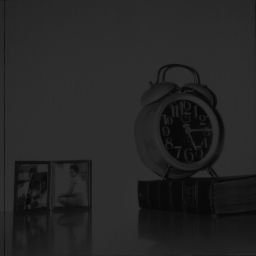
\includegraphics[width=0.3\textwidth]{1/1Gray_Const_Multipl_Result}
		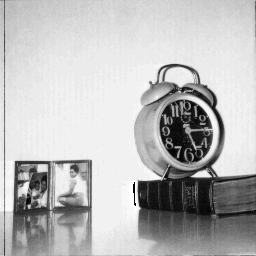
\includegraphics[width=0.3\textwidth]{1/1Gray_Const_Multipl_Result_Norm}
	\end{center}
	\caption{(Od lewej) Szary obraz wejściowy, obraz po przemnożeniu przez liczbę=50, obraz po normalizacji }
\end{figure}

\begin{figure}[H]
	\begin{center}
		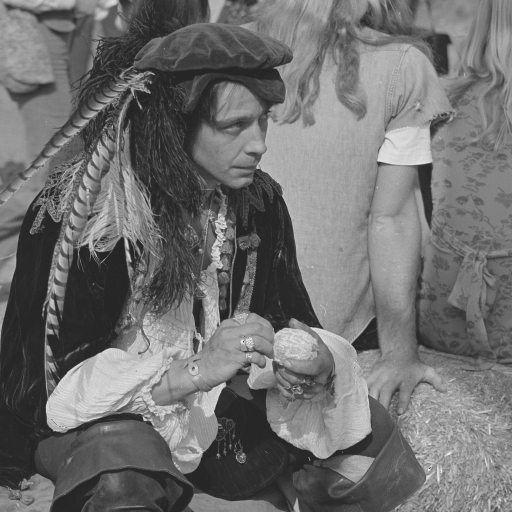
\includegraphics[width=0.3\textwidth]{2/2Gray_Const_Multipl_Original}
		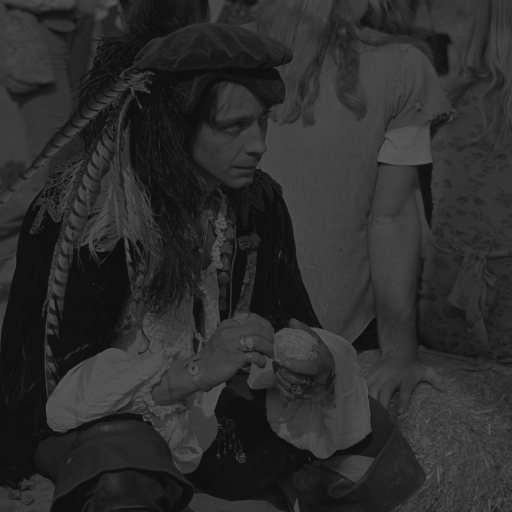
\includegraphics[width=0.3\textwidth]{2/2Gray_Const_Multipl_Result}
		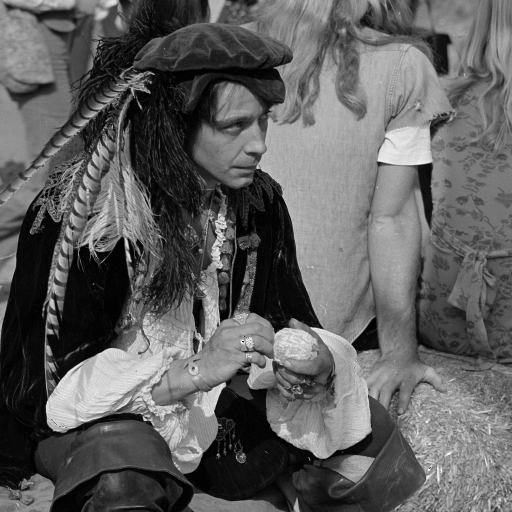
\includegraphics[width=0.3\textwidth]{2/2Gray_Const_Multipl_Result_Norm}
	\end{center}
	\caption{(Od lewej) Szary obraz wejściowy, obraz po przemnożeniu przez liczbę=100, obraz po normalizacji }
\end{figure}

\subsection*{Kod źródłowy}

\begin{lstlisting}[caption=Mnożenie obrazu szarego przez zadaną liczbę]

iimage1_matrix = self.im1
height = image1_matrix.shape[0]   # wysokosc
width = image1_matrix.shape[1]    # szereoksc

result_matrix = np.zeros((width, height), dtype=np.uint8)

# Inicjalizacja zmiennych
f_min = 255
f_max = 0

# Mnozenie 
for y in range(height):
    for x in range(width):  

        L = int(image1_matrix[x][y]) 
        if L == 255:
            L = const
        elif L == 0:
            L = 0
        else:
            L = (int(image1_matrix[x][y]) * const)/255 

        # Zaokroglenie do najblizszej wartosci calkowitej z gory
        # i przypisanie wartosci
        result_matrix[x][y] = math.ceil(L)

        # Poszukiwanie minimum i maksimum
        if f_min > L:
            f_min = L
        if f_max < L:
            f_max = L

# Normalizacja
norm_matrix = np.zeros((width, height), dtype=np.uint8)
for y in range(height):
    for x in range(width):
        norm_matrix[x][y] = 255 * ((result_matrix[x][y] - f_min) / (f_max - f_min))

\end{lstlisting}






\section {Mnożenie obrazu przez inny obraz}
\hfill
\\\\
\indent
\begin{figure}[H]
	\begin{center}
		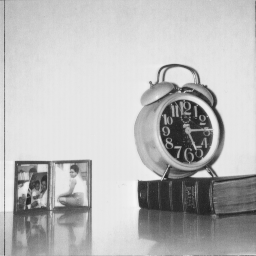
\includegraphics[width=0.3\textwidth]{1/1Gray_Img1_Multipl_Original}
		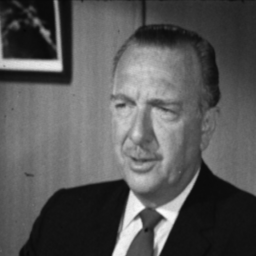
\includegraphics[width=0.3\textwidth]{1/1Gray_Img2_Multipl_Original}
		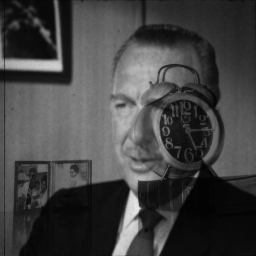
\includegraphics[width=0.3\textwidth]{1/1Gray_Img_Multipl_Result}
		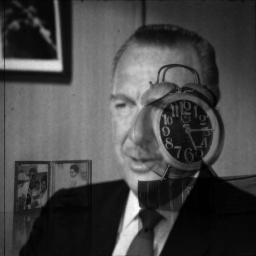
\includegraphics[width=0.3\textwidth]{1/1Gray_Img_Multipl_Result_Norm}
	\end{center}
	\caption{(Od lewej) Pierwsze dwa to szare obrazy wejściowe, następnie obraz powstały w wyniku przemnożenia obrazów, poniżej obraz wynikowy po normalizacji }
\end{figure}

\begin{figure}[H]
	\begin{center}
		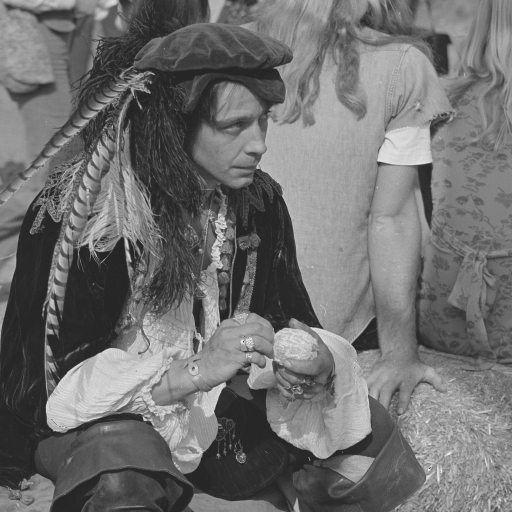
\includegraphics[width=0.3\textwidth]{2/2Gray_Img1_Multipl_Original}
		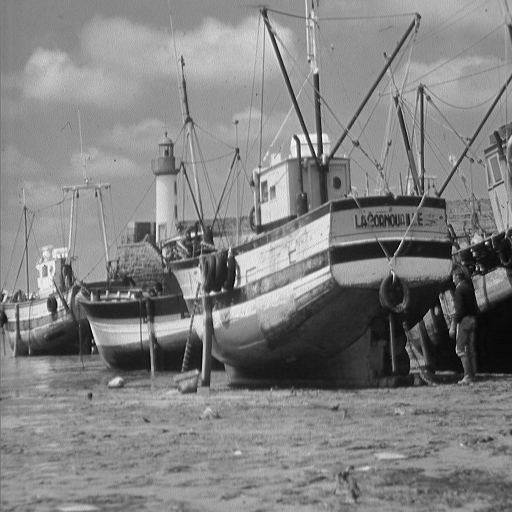
\includegraphics[width=0.3\textwidth]{2/2Gray_Img2_Multipl_Original}
		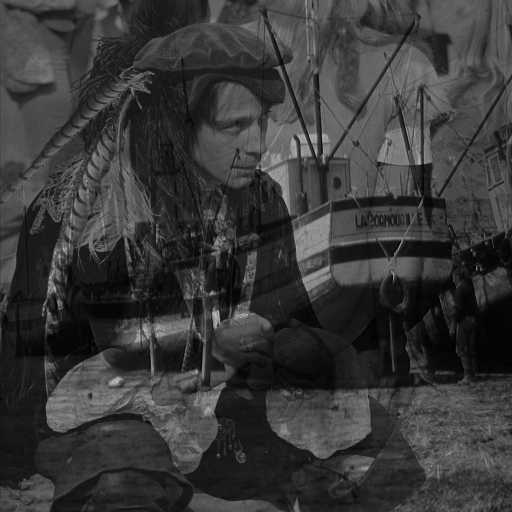
\includegraphics[width=0.3\textwidth]{2/2Gray_Img_Multipl_Result}
		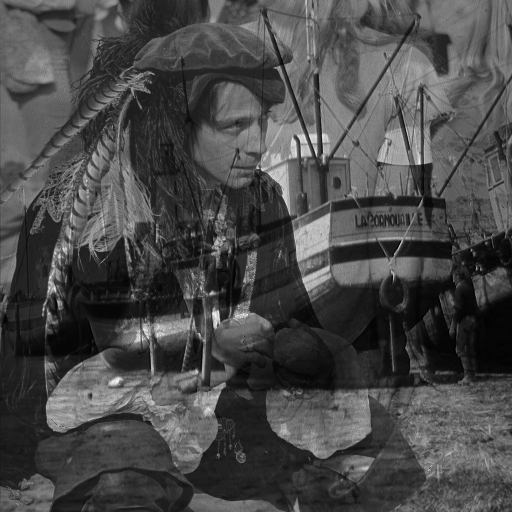
\includegraphics[width=0.3\textwidth]{2/2Gray_Img_Multipl_Result_Norm}
	\end{center}
	\caption{(Od lewej) Pierwsze dwa to szare obrazy wejściowe, następnie obraz powstały w wyniku przemnożenia obrazów, poniżej obraz wynikowy po normalizacji }
\end{figure}

\subsection*{Kod źródłowy}

\begin{lstlisting}[caption=Mnożenie obrazu szarego przez inny obraz ]

image1_matrix = self.im1
image2_matrix = self.im2
height = image1_matrix.shape[0]   # wysokosc
width = image1_matrix.shape[1]    # szereoksc

result_matrix = np.zeros((width, height), dtype=np.uint8)

# Inicjalizacja zmiennych
f_min = 255
f_max = 0

for y in range(height):
    for x in range(width):  

        L = int(image1_matrix[x][y]) 
        if L == 255:
            L = image2_matrix[x][y]
        elif L == 0:
            L = 0
        else:
            L = (int(image1_matrix[x][y]) * int(image2_matrix[x][y]))/255 

        # Zaokroglenie do najblizszej wartosci calkowitej z gory
        # i przypisanie wartosci
        result_matrix[x][y] = math.ceil(L)
                        
        # Poszukiwanie minimum i maksimum
        if f_min > L:
            f_min = L
        if f_max < L:
            f_max = L

# Normalizacja
norm_matrix = np.zeros((width, height), dtype=np.uint8)
for y in range(height):
    for x in range(width):
        norm_matrix[x][y] = 255 * ((result_matrix[x][y] - f_min) / (f_max - f_min))

\end{lstlisting}

%\section {Mnożenie obrazu przez zadaną liczbę oraz przez inny obraz}
\section {Mieszanie obrazów z określonym współczynnikiem}

\begin{figure}[H]
	\begin{center}
		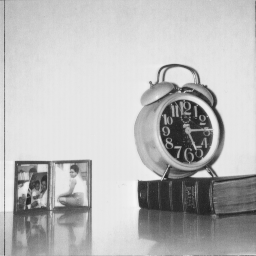
\includegraphics[width=0.3\textwidth]{1/1Gray_Img1_Mix_Original}
		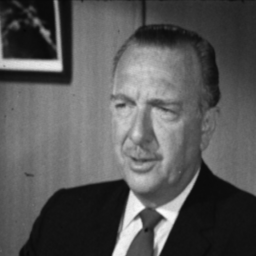
\includegraphics[width=0.3\textwidth]{1/1Gray_Img2_Mix_Original}
		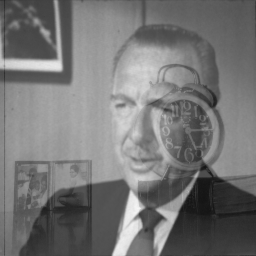
\includegraphics[width=0.3\textwidth]{1/1Gray_Img_Mix_Result}
		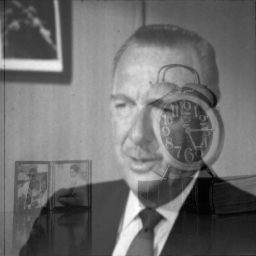
\includegraphics[width=0.3\textwidth]{1/1Gray_Img_Mix_Result_Norm}
	\end{center}
	\caption{(Od lewej) Dwa obrazy wejściowe, następnie obraz powstały w wyniku mieszania obrazów ze współczynnikiem $\alpha$=0.5, poniżej obraz wynikowy po normalizacji }
\end{figure}

\begin{figure}[H]
	\begin{center}
		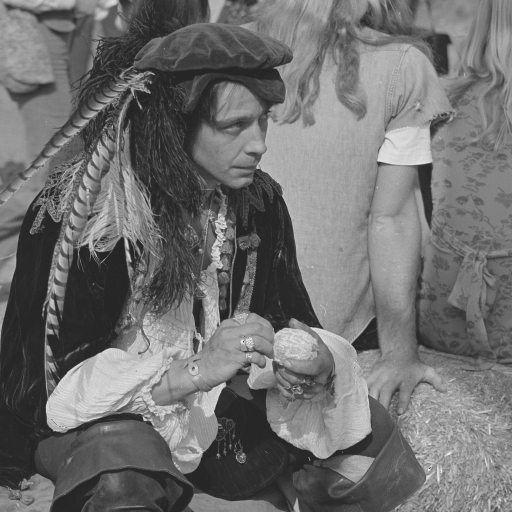
\includegraphics[width=0.3\textwidth]{2/2Gray_Img1_Mix_Original}
		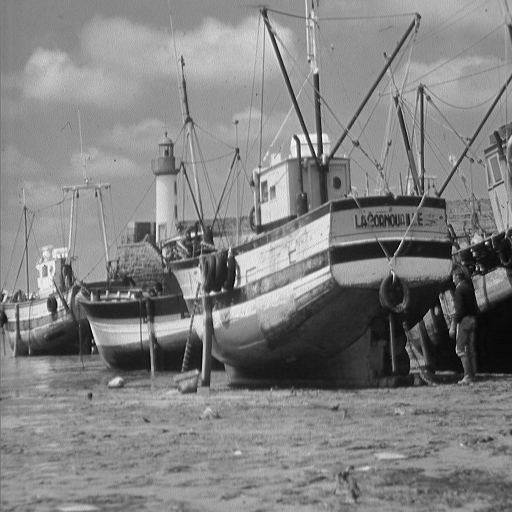
\includegraphics[width=0.3\textwidth]{2/2Gray_Img2_Mix_Original}
		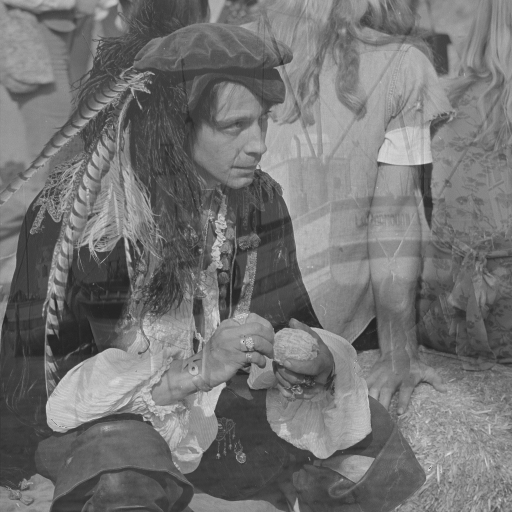
\includegraphics[width=0.3\textwidth]{2/2Gray_Img_Mix_Result}
		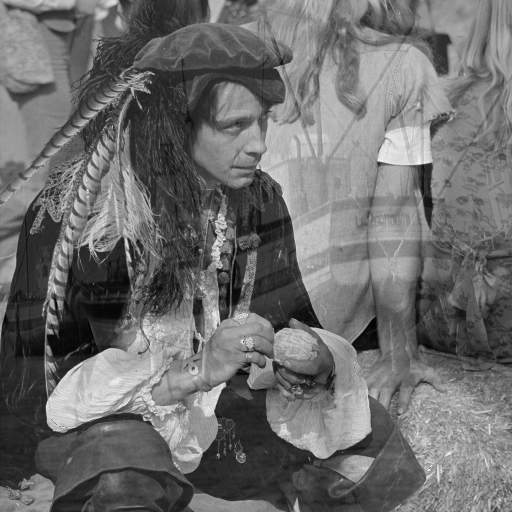
\includegraphics[width=0.3\textwidth]{2/2Gray_Img_Mix_Result_Norm}
	\end{center}
	\caption{(Od lewej) Dwa obrazy wejściowe, następnie obraz powstały w wyniku mieszania obrazów ze współczynnikiem $\alpha$=0.8, poniżej obraz wynikowy po normalizacji }
\end{figure}


\begin{lstlisting}[caption=Mieszanie obrazów szarych z określonym współczynnikiem]

image1_matrix = self.im1
image2_matrix = self.im2
height = image1_matrix.shape[0]   # wysokosc
width = image1_matrix.shape[1]    # szereoksc

result_matrix = np.zeros((width, height), dtype=np.uint8)

# Inicjalizacja zmiennych
f_min = 255
f_max = 0

for y in range(height):
    for x in range(width):  

        L = float(image1_matrix[x][y]) * alfa + (1-alfa) * float(image2_matrix[x][y])

        # Zaokroglenie do najblizszej wartosci calkowitej z gory
        # i przypisanie wartosci
        result_matrix[x][y] = math.ceil(L)

        # Poszukiwanie minimum i maksimum
        if f_min > L:
            f_min = L
        if f_max < L:
            f_max = L

# Normalizacja
norm_matrix = np.zeros((width, height), dtype=np.uint8)
for y in range(height):
    for x in range(width):
        norm_matrix[x][y] = 255 * ((result_matrix[x][y] - f_min) / (f_max - f_min))
        
\end{lstlisting}



\section {Potęgowanie obrazu (z zadaną potęgą)}

\hfill
\\\\
\indent

\begin{figure}[H]
	\begin{center}
		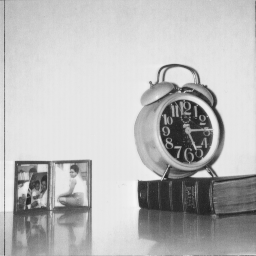
\includegraphics[width=0.3\textwidth]{1/1Gray_Pow_Original}
		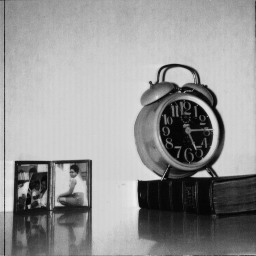
\includegraphics[width=0.3\textwidth]{1/1Gray_Pow_Result}
		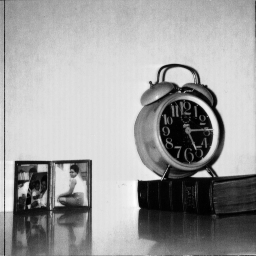
\includegraphics[width=0.3\textwidth]{1/1Gray_Pow_Result_Norm}
	\end{center}
	\caption{(Od lewej) Szary obraz wejściowy, obraz po podniesieniu do potęgi $\alpha$=2, obraz po normalizacji }
\end{figure}

\begin{figure}[H]
	\begin{center}
		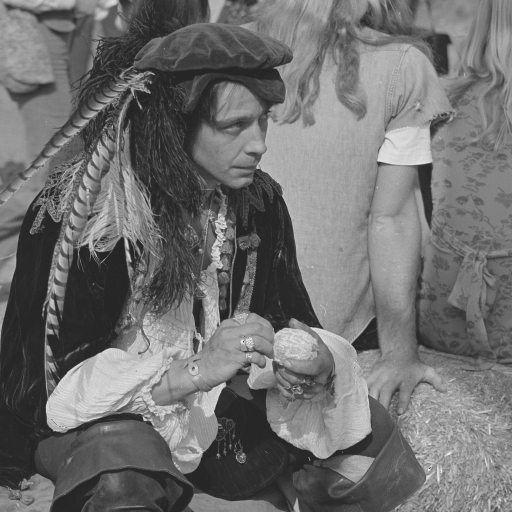
\includegraphics[width=0.3\textwidth]{2/2Gray_Pow_Original}
		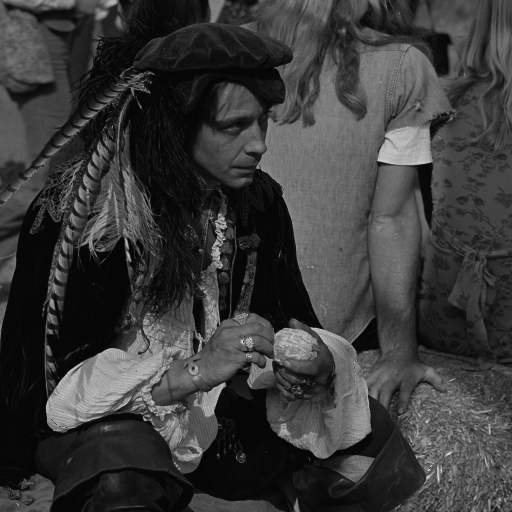
\includegraphics[width=0.3\textwidth]{2/2Gray_Pow_Result}
		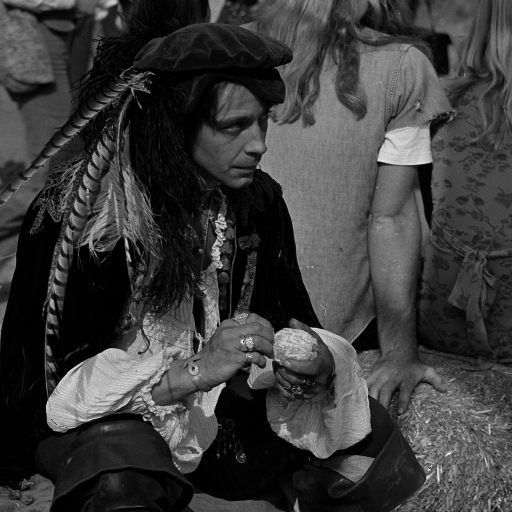
\includegraphics[width=0.3\textwidth]{2/2Gray_Pow_Result_Norm}
	\end{center}
	\caption{(Od lewej) Szary obraz wejściowy, obraz po podniesieniu do potęgi $\alpha$=3, obraz po normalizacji }
\end{figure}

\subsection*{Kod źródłowy}

\begin{lstlisting}[caption=Potęgowanie obrazu szarego (z zadaną potęgą)]

image_matrix = self.im1
height = image_matrix.shape[0]   # wysokosc
width = image_matrix.shape[1]    # szereoksc

result_matrix = np.zeros((width, height), dtype=np.uint8)

# Inicjalizacja zmiennych
f_min = 255
f_max = 0
f_img_max = 0

for y in range(height):
    for x in range(width):  
        
        L = int(image_matrix[x][y])

        # Poszukiwanie maksimum
        if f_img_max < L:
            f_img_max = L

for y in range(height):
    for x in range(width):  
        
        L = int(image_matrix[x][y])
        if L == 255:
            L = 255
        elif L == 0:
            L = 0
        else:
            L = math.pow(int(image_matrix[x][y]) / f_img_max, alfa) * 255

        # Zaokroglenie do najblizszej wartosci calkowitej z gory
        # i przypisanie wartosci
        result_matrix[x][y] = math.ceil(L)

        # Poszukiwanie minimum i maksimum
        if f_min > L:
            f_min = L
        if f_max < L:
            f_max = L

# Normalizacja
norm_matrix = np.zeros((width, height), dtype=np.uint8)
for y in range(height):
    for x in range(width):
        norm_matrix[x][y] = 255 * ((result_matrix[x][y] - f_min) / (f_max - f_min))



\end{lstlisting}

\section {Dzielenie obrazu przez (zadaną) liczbę }

\hfill
\\\\
\indent

\begin{figure}[H]
	\begin{center}
		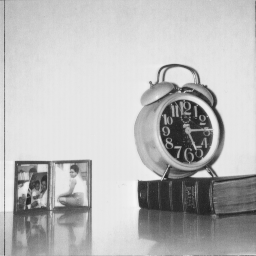
\includegraphics[width=0.3\textwidth]{1/1Gray_Div_Original}
		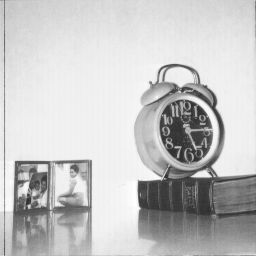
\includegraphics[width=0.3\textwidth]{1/1Gray_Div_Result}
		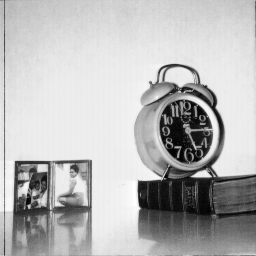
\includegraphics[width=0.3\textwidth]{1/1Gray_Div_Result_Norm}
	\end{center}
	\caption{(Od lewej) Szary obraz wejściowy, obraz po podzieleniu przez liczbę=15, obraz po normalizacji }
\end{figure}

\begin{figure}[H]
	\begin{center}
		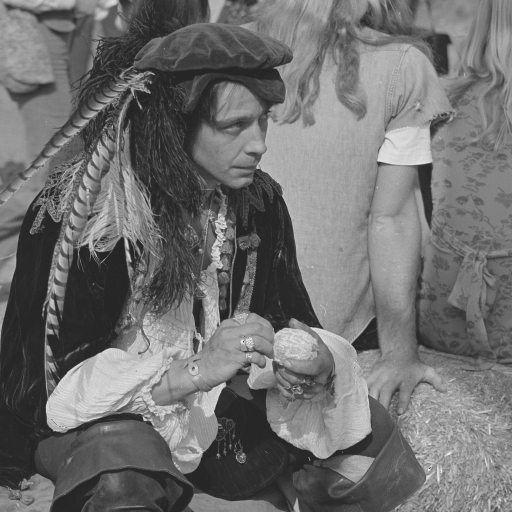
\includegraphics[width=0.3\textwidth]{2/2Gray_Div_Original}
		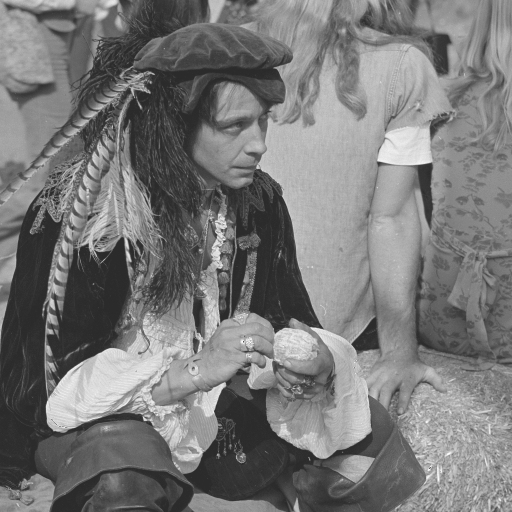
\includegraphics[width=0.3\textwidth]{2/2Gray_Div_Result}
		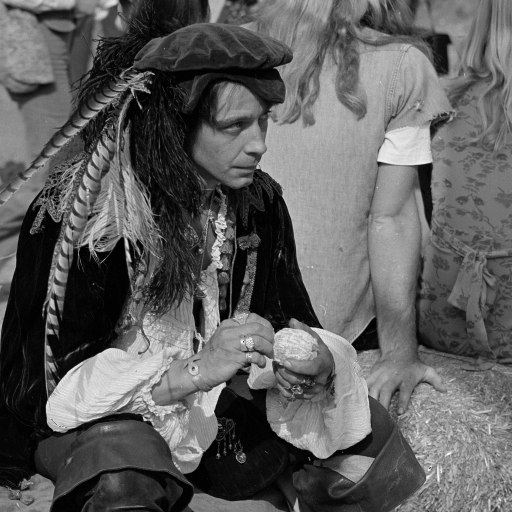
\includegraphics[width=0.3\textwidth]{2/2Gray_Div_Result_Norm}
	\end{center}
	\caption{(Od lewej) Szary obraz wejściowy, obraz po podzieleniu przez liczbę=3, obraz po normalizacji }
\end{figure}

\subsection*{Kod źródłowy}

\begin{lstlisting}[caption=Dzielenie obrazu szarego przez (zadaną) liczbę ]

image_matrix = self.im1
height = image_matrix.shape[0]   # wysokosc
width = image_matrix.shape[1]    # szereoksc

result_matrix = np.zeros((width, height), dtype=np.uint8)

# Inicjalizacja zmiennych
f_min = 255
f_max = 0
Q_max = 0

for y in range(height):
    for x in range(width):  

        L = int(image_matrix[x][y]) + int(const)

        # Poszukiwanie maksimum
        if Q_max < L:
            Q_max = L

for y in range(height):
    for x in range(width):  

        L = int(image_matrix[x][y]) + int(const)
        Q_L = (L * 255) / Q_max

        # Zaokroglenie do najblizszej wartosci calkowitej z gory
        # i przypisanie wartosci
        result_matrix[x][y] = math.ceil(Q_L)

        # Poszukiwanie minimum i maksimum
        if f_min > Q_L:
            f_min = Q_L
        if f_max < Q_L:
            f_max = Q_L

# Normalizacja
norm_matrix = np.zeros((width, height), dtype=np.uint8)
for y in range(height):
    for x in range(width):
        norm_matrix[x][y] = 255 * ((result_matrix[x][y] - f_min) / (f_max - f_min))
        
        
\end{lstlisting}

\section {Dzielenie obrazu przez przez inny obraz}

\hfill
\\\\
\indent

\begin{figure}[H]
	\begin{center}
		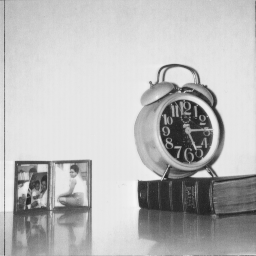
\includegraphics[width=0.3\textwidth]{1/1Gray_Img1_Div_Original}
		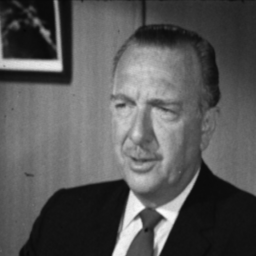
\includegraphics[width=0.3\textwidth]{1/1Gray_Img2_Div_Original}
		\includegraphics[width=0.3\textwidth]{1/1Gray_Img_Div_Result}
		\includegraphics[width=0.3\textwidth]{1/1Gray_Img_Div_Result_Norm}
	\end{center}
	\caption{(Od lewej) Dwa obrazy wejściowe, następnie obraz powstały w wyniku podzielenia obrazów, poniżej obraz wynikowy po normalizacji }
\end{figure}

\begin{figure}[H]
	\begin{center}
		\includegraphics[width=0.3\textwidth]{2/2Gray_Img1_Div_Original}
		\includegraphics[width=0.3\textwidth]{2/2Gray_Img2_Div_Original}
		\includegraphics[width=0.3\textwidth]{2/2Gray_Img_Div_Result}
		\includegraphics[width=0.3\textwidth]{2/2Gray_Img_Div_Result_Norm}
	\end{center}
	\caption{(Od lewej) Dwa obrazy wejściowe, następnie obraz powstały w wyniku podzielenia obrazów, poniżej obraz wynikowy po normalizacji }
\end{figure}


\begin{lstlisting}[caption=Dzielenie obrazu szarego przez przez inny obraz]

image1_matrix = self.im1
image2_matrix = self.im2
height = image1_matrix.shape[0]   # wysokosc
width = image1_matrix.shape[1]    # szereoksc

result_matrix = np.zeros((width, height), dtype=np.uint8)

# Inicjalizacja zmiennych
f_min = 255
f_max = 0
Q_max = 0

for y in range(height):
    for x in range(width):  
        # Obliczanie sumy
        L = int(image1_matrix[x][y]) + int(image2_matrix[x][y])
        
        # Poszukiwanie maksimum
        if Q_max < L:
            Q_max = L

for y in range(height):
    for x in range(width):  

        # Obliczanie sumy
        L = int(image1_matrix[x][y]) + int(image2_matrix[x][y])
        Q_L = (L * 255) / Q_max

        # Zaokroglenie do najblizszej wartosci calkowitej z gory
        # i przypisanie wartosci
        result_matrix[x][y] = math.ceil(Q_L)

        # Poszukiwanie minimum i maksimum
        if f_min > Q_L:
            f_min = Q_L
        if f_max < Q_L:
            f_max = Q_L

# Normalizacja
norm_matrix = np.zeros((width, height), dtype=np.uint8)
for y in range(height):
    for x in range(width):
        norm_matrix[x][y] = 255 * ((result_matrix[x][y] - f_min) / (f_max - f_min))

\end{lstlisting}


\section {Pierwiastkowanie obrazu}
\hfill
\\\\
\indent

\begin{figure}[H]
	\begin{center}
		\includegraphics[width=0.3\textwidth]{1/1Gray_Sqrt_Original}
		\includegraphics[width=0.3\textwidth]{1/1Gray_Sqrt_Result}
		\includegraphics[width=0.3\textwidth]{1/1Gray_Sqrt_Result_Norm}
	\end{center}
	\caption{(Od lewej) Szary obraz wejściowy, obraz po spierwiastkowaniu pierwiastkiem kwadratowym ($\alpha$=1/2), obraz po normalizacji }
\end{figure}

\begin{figure}[H]
	\begin{center}
		\includegraphics[width=0.3\textwidth]{2/2Gray_Sqrt_Original}
		\includegraphics[width=0.3\textwidth]{2/2Gray_Sqrt_Result}
		\includegraphics[width=0.3\textwidth]{2/2Gray_Sqrt_Result_Norm}
	\end{center}
	\caption{(Od lewej) Szary obraz wejściowy, obraz po spierwiastkowaniu pierwiastkiem stopnia trzeciego ($\alpha$=1/3), obraz po normalizacji }
\end{figure}

\subsection*{Kod źródłowy}

\begin{lstlisting}[caption=Pierwiastkowanie obrazu szarego]

image_matrix = self.im1
height = image_matrix.shape[0]   # wysokosc
width = image_matrix.shape[1]    # szereoksc

result_matrix = np.zeros((width, height), dtype=np.uint8)

# Inicjalizacja zmiennych
f_min = 255
f_max = 0
f_img_max = 0

alfa = 1/deg # Zamiana stopnia pierwiastka na ulamek

for y in range(height):
    for x in range(width):  
        
        L = int(image_matrix[x][y])

        # Poszukiwanie maksimum
        if f_img_max < L:
            f_img_max = L

for y in range(height):
    for x in range(width):  
        
        L = int(image_matrix[x][y])
        if L == 255:
            L = 255
        elif L == 0:
            L = 0
        else:
            L = math.pow(int(image_matrix[x][y]) / f_img_max, alfa) * 255

        # Zaokroglenie do najblizszej wartosci calkowitej z gory
        # i przypisanie wartosci
        result_matrix[x][y] = math.ceil(L)

        # Poszukiwanie minimum i maksimum
        if f_min > L:
            f_min = L
        if f_max < L:
            f_max = L

# Normalizacja
norm_matrix = np.zeros((width, height), dtype=np.uint8)
for y in range(height):
    for x in range(width):
        norm_matrix[x][y] = 255 * ((result_matrix[x][y] - f_min) / (f_max - f_min))

\end{lstlisting}

\section {Logarytmowanie obrazu}

\hfill
\\\\
\indent

\begin{figure}[H]
	\begin{center}
		\includegraphics[width=0.3\textwidth]{1/1Gray_Log_Original}
		\includegraphics[width=0.3\textwidth]{1/1Gray_Log_Result}
		\includegraphics[width=0.3\textwidth]{1/1Gray_Log_Result_Norm}
	\end{center}
	\caption{(Od lewej) Szary obraz wejściowy, obraz po logarytmowaniu logarytmem naturalnym, obraz po normalizacji }
\end{figure}

\begin{figure}[H]
	\begin{center}
		\includegraphics[width=0.3\textwidth]{2/2Gray_Log_Original}
		\includegraphics[width=0.3\textwidth]{2/2Gray_Log_Result}
		\includegraphics[width=0.3\textwidth]{2/2Gray_Log_Result_Norm}
	\end{center}
	\caption{(Od lewej) Szary obraz wejściowy, obraz po logarytmowaniu logarytmem naturalnym, obraz po normalizacji }
\end{figure}

\subsection*{Kod źródłowy}

\begin{lstlisting}[caption=Logarytmowanie obrazu szarego]

image_matrix = self.im1
height = image_matrix.shape[0]   # wysokosc
width = image_matrix.shape[1]    # szereoksc

result_matrix = np.zeros((width, height), dtype=np.uint8)

# Inicjalizacja zmiennych
f_min = 255
f_max = 0
f_img_max = 0

for y in range(height):
    for x in range(width):  

        L = int(image_matrix[x][y]) 

        # Poszukiwanie maksimum
        if f_img_max < L:
            f_img_max = L

for y in range(height):
    for x in range(width):  

        L = int(image_matrix[x][y]) 

        if L == 0:
            L = 0
        else:
            L = (math.log(1 + L) / math.log(1 + f_img_max)) * 255

        # Zaokroglenie do najblizszej wartosci calkowitej z gory
        # i przypisanie wartosci
        result_matrix[x][y] = math.ceil(L)

        # Poszukiwanie minimum i maksimum
        if f_min > L:
            f_min = L
        if f_max < L:
            f_max = L

# Normalizacja
norm_matrix = np.zeros((width, height), dtype=np.uint8)
for y in range(height):
    for x in range(width):
        norm_matrix[x][y] = 255 * ((result_matrix[x][y] - f_min) / (f_max - f_min))


\end{lstlisting}


\chapter{Operacje sumowania arytmetycznego obrazów barwowych}

Arytmetyczne operacje na obrazach barwowych przeprowadza się wykonując działania na pojedynczych pikslach i są uwarunkowane wymaganiami zależnymi od typu operacji. 
W przedstawionych zadaniach poruszamy się w przestrzeni barw RGB, a do normalizacji wykorzystano wzór:

	\begin{center}
		$ f_{norm} = Z_{rep}[(f - f_{min}) / (f_{max} - f_{min})] $
	\end{center}


\section{Sumowanie (określonej) stałej z obrazem}
\hfill
\\\\
\indent
Algorytm sumowania obrazu barwowego z określoną stałą polega na dodaniu do każdej składowej barwowej pojedynczego piksla stałej liczby.
Po operacji sumowania następuje normalizacja obrazu.

	\begin{enumerate}	
		\item Policz sumy wartości kazdego piksla ze stałą ($const$).
		\item Jeżeli jedna z tych sum jest większa niż 255 to:
		\item Wybierz największą sumę  $Q_{max}$ i policz $D_{max}$ ze wzoru: $D_{max}[i,j] = (Q_{max}[i,j] - 255)$ 
		\item Oblicz $X = D_{max} / 255$
		\item Policz sumy ze wzoru
		\begin{center}$Q_{R}[i,j] = P_{R}[i,j] - (P_{1R} * X)+ const - (const * X) -1$ \\
			$Q_{G}[i,j] = P_{G}[i,j] - (P_{G} * X)+ const - (const * X) -1$ \\
			$Q_{B}[i,j] = P_{B}[i,j] - (P_{B} * X)+ const - (const * X) -1$
		\end{center}
	\end{enumerate}

\begin{figure}[H]
	\begin{center}
		\includegraphics[width=0.3\textwidth]{1/1Color_Const_Sum_Original}
		\includegraphics[width=0.3\textwidth]{1/1Color_Const_Sum_Result}
		\includegraphics[width=0.3\textwidth]{1/1Color_Const_Sum_Result_Norm}
	\end{center}
	\caption{(Od lewej) Barwowy obraz wejściowy, obraz po sumowaniu ze stałą = 50, obraz po normalizacji }
\end{figure}

\begin{figure}[H]
	\begin{center}
		\includegraphics[width=0.3\textwidth]{2/2Color_Const_Sum_Original}
		\includegraphics[width=0.3\textwidth]{2/2Color_Const_Sum_Result}
		\includegraphics[width=0.3\textwidth]{2/2Color_Const_Sum_Result_Norm}
	\end{center}
	\caption{(Od lewej) Barwowy obraz wejściowy, obraz po sumowaniu ze stałą = 100, obraz po normalizacji }
\end{figure}

\begin{lstlisting}[caption=Sumowanie obrazu barwowego ze stałą]

image_matrix = self.im1
height = image_matrix.shape[0]   # wysokosc
width = image_matrix.shape[1]    # szereoksc

result_matrix = np.zeros((width, height, 3), dtype=np.uint8)

# Inicjalizacja zmiennych
Q_max = 0
D_max = 0
X = 0
f_min = 255
f_max = 0

for y in range(height):
    for x in range(width):  

        # Obliczanie sum
        R = int(image_matrix[x][y][0]) + int(const)
        G = int(image_matrix[x][y][1]) + int(const)
        B = int(image_matrix[x][y][2]) + int(const)

        # Poszukiwanie maksimum               
        if Q_max < max([R, G, B]):
            Q_max = max([R, G, B])

# Sprawdzenie czy maksimum przekracza zakres
if Q_max > 255:
    D_max = Q_max - 255
    X = (D_max/255) # Obliczenie proporcji

# Obliczenie sum z uwzglednieniem zakresu
for y in range(height):
    for x in range(width): 
        R = (image_matrix[x][y][0] - (image_matrix[x][y][0] * X)) + (const - (const * X))
        G = (image_matrix[x][y][1] - (image_matrix[x][y][1] * X)) + (const - (const * X))
        B = (image_matrix[x][y][2] - (image_matrix[x][y][2] * X)) + (const - (const * X))

        # Zaokroglenie do najblizszej wartosci calkowitej z gory
        # i przypisanie wartosci
        result_matrix[x][y][0] = math.ceil(R)
        result_matrix[x][y][1] = math.ceil(G)
        result_matrix[x][y][2] = math.ceil(B)

        # Poszukiwanie minimum i maksimum                
        if f_min > min([R, G, B]):
            f_min = min([R, G, B])
        if f_max < max([R, G, B]):
            f_max = max([R, G, B])

# Normalizacja
norm_matrix = np.zeros((width, height, 3), dtype=np.uint8)
for y in range(height):
    for x in range(width):
        norm_matrix[x][y][0] = 255 * ((result_matrix[x][y][0] - f_min) / (f_max - f_min))
        norm_matrix[x][y][1] = 255 * ((result_matrix[x][y][1] - f_min) / (f_max - f_min))
        norm_matrix[x][y][2] = 255 * ((result_matrix[x][y][2] - f_min) / (f_max - f_min))

\end{lstlisting}

\section {Sumowanie dwóch obrazów}
\hfill
\\\\
\indent

\begin{figure}[H]
	\begin{center}
		\includegraphics[width=0.3\textwidth]{1/1Color_Sum_Img1_Original}
		\includegraphics[width=0.3\textwidth]{1/1Color_Sum_Img2_Original}
		\includegraphics[width=0.3\textwidth]{1/1Color_Sum_Img_Result}
		\includegraphics[width=0.3\textwidth]{1/1Color_Sum_Img_Result_Norm}
	\end{center}
	\caption{(Od lewej) Pierwsze dwa to barwowe obrazy wejściowe, następnie obraz powstały w wyniku sumowania obrazów, poniżej obraz wynikowy po normalizacji }
\end{figure}

\begin{figure}[H]
	\begin{center}
		\includegraphics[width=0.3\textwidth]{2/2Color_Sum_Img1_Original}
		\includegraphics[width=0.3\textwidth]{2/2Color_Sum_Img2_Original}
		\includegraphics[width=0.3\textwidth]{2/2Color_Sum_Img_Result}
		\includegraphics[width=0.3\textwidth]{2/2Color_Sum_Img_Result_Norm}
	\end{center}
	\caption{(Od lewej) Pierwsze dwa to barwowe obrazy wejściowe, następnie obraz powstały w wyniku sumowania obrazów, poniżej obraz wynikowy po normalizacji }
\end{figure}


\begin{lstlisting}[caption=Sumowanie obrazów barwowych]

image1_matrix = self.im1
image2_matrix = self.im2
height = image1_matrix.shape[0]   # wysokosc
width = image1_matrix.shape[1]    # szereoksc

result_matrix = np.zeros((width, height, 3), dtype=np.uint8)

# Inicjalizacja zmiennych
Q_max = 0
D_max = 0
X = 0
f_min = 255
f_max = 0

for y in range(height):
    for x in range(width):  

        # Obliczanie sum
        R = int(image1_matrix[x][y][0]) + int(image2_matrix[x][y][0])
        G = int(image1_matrix[x][y][1]) + int(image2_matrix[x][y][1])
        B = int(image1_matrix[x][y][2]) + int(image2_matrix[x][y][2])
        
        # Poszukiwanie maksimum               
        if Q_max < max([R, G, B]):
            Q_max = max([R, G, B])

# Sprawdzenie czy maximum przekracza zakres
if Q_max > 255:
    D_max = Q_max - 255
    X = (D_max/255) # Obliczenie proporcji

# Obliczenie sum z uwzglednieniem zakresu
for y in range(height):
    for x in range(width): 
        R = (image1_matrix[x][y][0] - (image1_matrix[x][y][0] * X)) + (image2_matrix[x][y][0] - (image2_matrix[x][y][0] * X))
        G = (image1_matrix[x][y][1] - (image1_matrix[x][y][1] * X)) + (image2_matrix[x][y][1] - (image2_matrix[x][y][1] * X))
        B = (image1_matrix[x][y][2] - (image1_matrix[x][y][2] * X)) + (image2_matrix[x][y][2] - (image2_matrix[x][y][2] * X))

        # Zaokroglenie do najblizszej wartosci calkowitej z gory
        # i przypisanie wartosci
        result_matrix[x][y][0] = math.ceil(R)
        result_matrix[x][y][1] = math.ceil(G)
        result_matrix[x][y][2] = math.ceil(B)

        # Poszukiwanie minimum i maksimum                
        if f_min > min([R, G, B]):
            f_min = min([R, G, B])
        if f_max < max([R, G, B]):
            f_max = max([R, G, B])

# Normalizacja
norm_matrix = np.zeros((width, height, 3), dtype=np.uint8)
for y in range(height):
    for x in range(width):
        norm_matrix[x][y][0] = 255 * ((result_matrix[x][y][0] - f_min) / (f_max - f_min))
        norm_matrix[x][y][1] = 255 * ((result_matrix[x][y][1] - f_min) / (f_max - f_min))
        norm_matrix[x][y][2] = 255 * ((result_matrix[x][y][2] - f_min) / (f_max - f_min))

\end{lstlisting}

\section {Mnożenie obrazu przez zadaną liczbę}
\hfill
\\\\
\indent

\begin{figure}[H]
	\begin{center}
		\includegraphics[width=0.3\textwidth]{1/1Color_Const_Multipl_Original}
		\includegraphics[width=0.3\textwidth]{1/1Color_Const_Multipl_Result}
		\includegraphics[width=0.3\textwidth]{1/1Color_Const_Multipl_Result_Norm}
	\end{center}
	\caption{(Od lewej) Szary obraz wejściowy, obraz po przemnożeniu przez liczbę 50, obraz po normalizacji }
\end{figure}

\begin{figure}[H]
	\begin{center}
		\includegraphics[width=0.3\textwidth]{2/2Color_Const_Multipl_Original}
		\includegraphics[width=0.3\textwidth]{2/2Color_Const_Multipl_Result}
		\includegraphics[width=0.3\textwidth]{2/2Color_Const_Multipl_Result_Norm}
	\end{center}
	\caption{(Od lewej) Szary obraz wejściowy, obraz po przemnożeniu przez liczbę 100, obraz po normalizacji }

\end{figure}

\subsection*{Kod źródłowy}

\begin{lstlisting}[caption=Mnożenie obrazu barwowego przez zadaną liczbę]

image_matrix = self.im1
height = image_matrix.shape[0]   # wysokosc
width = image_matrix.shape[1]    # szereoksc

result_matrix = np.zeros((width, height, 3), dtype=np.uint8)

# Inicjalizacja zmiennych
f_min = 255
f_max = 0

for y in range(height):
    for x in range(width):  

        R = int(image_matrix[x][y][0])
        G = int(image_matrix[x][y][1])
        B = int(image_matrix[x][y][2])

        if R == 255:
            R = const
        elif R == 0:
            R = 0
        else:
            R = (int(image_matrix[x][y][0]) * int(const))/255 
        
        if G == 255:
            G = const
        elif G == 0:
            G = 0
        else:
            G = (int(image_matrix[x][y][1]) * int(const))/255 
        
        if B == 255:
            B = const
        elif B == 0:
            B = 0
        else:
            B = (int(image_matrix[x][y][2]) * int(const))/255 

        # Zaokroglenie do najblizszej wartosci calkowitej z gory
        # i przypisanie wartosci
        result_matrix[x][y][0] = math.ceil(R)
        result_matrix[x][y][1] = math.ceil(G)
        result_matrix[x][y][2] = math.ceil(B)

        # Poszukiwanie minimum i maksimum                
        if f_min > min([R, G, B]):
            f_min = min([R, G, B])
        if f_max < max([R, G, B]):
            f_max = max([R, G, B])

# Normalizacja
norm_matrix = np.zeros((width, height, 3), dtype=np.uint8)
for y in range(height):
    for x in range(width):
        norm_matrix[x][y][0] = 255 * ((result_matrix[x][y][0] - f_min) / (f_max - f_min))
        norm_matrix[x][y][1] = 255 * ((result_matrix[x][y][1] - f_min) / (f_max - f_min))
        norm_matrix[x][y][2] = 255 * ((result_matrix[x][y][2] - f_min) / (f_max - f_min))


\end{lstlisting}

\section {Mnożenie obrazu przez inny obraz}
\hfill
\\\\
\indent


\begin{figure}[H]
	\begin{center}
		\includegraphics[width=0.3\textwidth]{1/1Color_Multipl_Img1_Original}
		\includegraphics[width=0.3\textwidth]{1/1Color_Multipl_Img2_Original}
		\includegraphics[width=0.3\textwidth]{1/1Color_Multipl_Img_Result}
		\includegraphics[width=0.3\textwidth]{1/1Color_Multipl_Img_Result_Norm}
	\end{center}
	\caption{(Od lewej) Pierwsze dwa to barwowe obrazy wejściowe, następnie obraz powstały w wyniku przemnożenia obrazów, poniżej obraz wynikowy po normalizacji }
\end{figure}

\begin{figure}[H]
	\begin{center}
		\includegraphics[width=0.3\textwidth]{2/2Color_Multipl_Img1_Original}
		\includegraphics[width=0.3\textwidth]{2/2Color_Multipl_Img2_Original}
		\includegraphics[width=0.3\textwidth]{2/2Color_Multipl_Img_Result}
		\includegraphics[width=0.3\textwidth]{2/2Color_Multipl_Img_Result_Norm}
	\end{center}
	\caption{(Od lewej) Pierwsze dwa to barwowe obrazy wejściowe, następnie obraz powstały w wyniku przemnożenia obrazów, poniżej obraz wynikowy po normalizacji }
\end{figure}

\subsection*{Kod źródłowy}

\begin{lstlisting}[caption=Mnożenie obrazu barwowego przez inny obraz ]

image1_matrix = self.im1
image2_matrix = self.im2
height = image1_matrix.shape[0]   # wysokosc
width = image1_matrix.shape[1]    # szereoksc

result_matrix = np.zeros((width, height, 3), dtype=np.uint8)

# Inicjalizacja zmiennych
f_min = 255
f_max = 0

for y in range(height):
    for x in range(width):  

        R = int(image1_matrix[x][y][0])
        G = int(image1_matrix[x][y][1])
        B = int(image1_matrix[x][y][2])

        if R == 255:
            R = image2_matrix[x][y][0]
        elif R == 0:
            R = 0
        else:
            R = (int(image1_matrix[x][y][0]) * int(image2_matrix[x][y][0]))/255 
        
        if G == 255:
            G = image2_matrix[x][y][1]
        elif G == 0:
            G = 0
        else:
            G = (int(image1_matrix[x][y][1]) * int(image2_matrix[x][y][1]))/255 
        
        if B == 255:
            B = image2_matrix[x][y][2]
        elif B == 0:
            B = 0
        else:
            B = (int(image1_matrix[x][y][2]) * int(image2_matrix[x][y][2]))/255 

        # Zaokroglenie do najblizszej wartosci calkowitej z gory
        # i przypisanie wartosci
        result_matrix[x][y][0] = math.ceil(R)
        result_matrix[x][y][1] = math.ceil(G)
        result_matrix[x][y][2] = math.ceil(B)

        # Poszukiwanie minimum i maksimum                
        if f_min > min([R, G, B]):
            f_min = min([R, G, B])
        if f_max < max([R, G, B]):
            f_max = max([R, G, B])

# Normalizacja
norm_matrix = np.zeros((width, height, 3), dtype=np.uint8)
for y in range(height):
    for x in range(width):
        norm_matrix[x][y][0] = 255 * ((result_matrix[x][y][0] - f_min) / (f_max - f_min))
        norm_matrix[x][y][1] = 255 * ((result_matrix[x][y][1] - f_min) / (f_max - f_min))
        norm_matrix[x][y][2] = 255 * ((result_matrix[x][y][2] - f_min) / (f_max - f_min))


\end{lstlisting}


\section{ Mieszanie obrazów z określonym współczynnikiem}

\hfill
\\\\
\indent

\begin{figure}[H]
	\begin{center}
		\includegraphics[width=0.3\textwidth]{1/1Color_Mix_Img1_Original}
		\includegraphics[width=0.3\textwidth]{1/1Color_Mix_Img2_Original}
		\includegraphics[width=0.3\textwidth]{1/1Color_Mix_Img_Result}
		\includegraphics[width=0.3\textwidth]{1/1Color_Mix_Img_Result_Norm}
	\end{center}
	\caption{(Od lewej) Dwa obrazy wejściowe, następnie obraz powstały w wyniku mieszania obrazów ze współczynnikiem $\alpha$=0.5, poniżej obraz wynikowy po normalizacji }
\end{figure}

\begin{figure}[H]
	\begin{center}
		\includegraphics[width=0.3\textwidth]{2/2Color_Mix_Img1_Original}
		\includegraphics[width=0.3\textwidth]{2/2Color_Mix_Img2_Original}
		\includegraphics[width=0.3\textwidth]{2/2Color_Mix_Img_Result}
		\includegraphics[width=0.3\textwidth]{2/2Color_Mix_Img_Result_Norm}
	\end{center}
	\caption{(Od lewej) Dwa obrazy wejściowe, następnie obraz powstały w wyniku mieszania obrazów ze współczynnikiem $\alpha$=0.8, poniżej obraz wynikowy po normalizacji }
\end{figure}

\begin{lstlisting}[caption=Mieszanie obrazów barwowych z określonym współczynnikiem]

image1_matrix = self.im1
image2_matrix = self.im2
height = image1_matrix.shape[0]   # wysokosc
width = image1_matrix.shape[1]    # szereoksc

result_matrix = np.zeros((width, height, 3), dtype=np.uint8)

# Inicjalizacja zmiennych
f_min = 255
f_max = 0

for y in range(height):
    for x in range(width):  

        R = float(image1_matrix[x][y][0]) * alfa + (1-alfa) * float(image2_matrix[x][y][0])
        G = float(image1_matrix[x][y][1]) * alfa + (1-alfa) * float(image2_matrix[x][y][1])
        B = float(image1_matrix[x][y][2]) * alfa + (1-alfa) * float(image2_matrix[x][y][2])

        # Zaokroglenie do najblizszej wartosci calkowitej z gory
        # i przypisanie wartosci
        result_matrix[x][y][0] = math.ceil(R)
        result_matrix[x][y][1] = math.ceil(G)
        result_matrix[x][y][2] = math.ceil(B)

        # Poszukiwanie minimum i maksimum                
        if f_min > min([R, G, B]):
            f_min = min([R, G, B])
        if f_max < max([R, G, B]):
            f_max = max([R, G, B])

# Normalizacja
norm_matrix = np.zeros((width, height, 3), dtype=np.uint8)
for y in range(height):
    for x in range(width):
        norm_matrix[x][y][0] = 255 * ((result_matrix[x][y][0] - f_min) / (f_max - f_min))
        norm_matrix[x][y][1] = 255 * ((result_matrix[x][y][1] - f_min) / (f_max - f_min))
        norm_matrix[x][y][2] = 255 * ((result_matrix[x][y][2] - f_min) / (f_max - f_min))


\end{lstlisting}

\section{ Potęgowanie obrazu}

\hfill
\\\\
\indent

\begin{figure}[H]
	\begin{center}
		\includegraphics[width=0.3\textwidth]{1/1Color_Pow_Original}
		\includegraphics[width=0.3\textwidth]{1/1Color_Pow_Result}
		\includegraphics[width=0.3\textwidth]{1/1Color_Pow_Result_Norm}
	\end{center}
	\caption{(Od lewej) Barwowy obraz wejściowy, obraz po podniesieniu do potęgi $\alpha$=2, obraz po normalizacji }
\end{figure}

\begin{figure}[H]
	\begin{center}
		\includegraphics[width=0.3\textwidth]{2/2Color_Pow_Original}
		\includegraphics[width=0.3\textwidth]{2/2Color_Pow_Result}
		\includegraphics[width=0.3\textwidth]{2/2Color_Pow_Result_Norm}
	\end{center}
	\caption{(Od lewej) Barwowy obraz wejściowy, obraz po podniesieniu do potęgi $\alpha$=3, obraz po normalizacji }
\end{figure}

\subsection*{Kod źródłowy}

\begin{lstlisting}[caption= Potęgowanie obrazu barwowego]

image1_matrix = self.im1
height = image1_matrix.shape[0]   # wysokosc
width = image1_matrix.shape[1]    # szereoksc

result_matrix = np.zeros((width, height, 3), dtype=np.uint8)

# Inicjalizacja zmiennych
f_min = 255
f_max = 0
f_img_max = 0

for y in range(height):
    for x in range(width):  

        R = int(image1_matrix[x][y][0])
        G = int(image1_matrix[x][y][1])
        B = int(image1_matrix[x][y][2])

        if f_img_max < max([R, G, B]):
            f_img_max = max([R, G, B])

for y in range(height):
    for x in range(width):  

        R = int(image1_matrix[x][y][0])
        G = int(image1_matrix[x][y][1])
        B = int(image1_matrix[x][y][2])

        if R == 0:
            R = 0
        else:
            R = 255 * (math.pow(int(image1_matrix[x][y][0]) / f_img_max, alfa))

        if G == 0:
            G = 0
        else:
            G = 255 * (math.pow(int(image1_matrix[x][y][1]) / f_img_max, alfa))
        
        if B == 0:
            B = 0
        else:
            B = 255 * (math.pow(int(image1_matrix[x][y][2]) / f_img_max, alfa))

        # Zaokroglenie do najblizszej wartosci calkowitej z gory
        # i przypisanie wartosci
        result_matrix[x][y][0] = math.ceil(R)
        result_matrix[x][y][1] = math.ceil(G)
        result_matrix[x][y][2] = math.ceil(B)

        # Poszukiwanie minimum i maksimum                
        if f_min > min([R, G, B]):
            f_min = min([R, G, B])
        if f_max < max([R, G, B]):
            f_max = max([R, G, B])

# Normalizacja
norm_matrix = np.zeros((width, height, 3), dtype=np.uint8)
for y in range(height):
    for x in range(width):
        norm_matrix[x][y][0] = 255 * ((result_matrix[x][y][0] - f_min) / (f_max - f_min))
        norm_matrix[x][y][1] = 255 * ((result_matrix[x][y][1] - f_min) / (f_max - f_min))
        norm_matrix[x][y][2] = 255 * ((result_matrix[x][y][2] - f_min) / (f_max - f_min))


\end{lstlisting}


\section{ Dzielenie obrazu przez (zadaną) liczbę}

\hfill
\\\\
\indent

\begin{figure}[H]
	\begin{center}
		\includegraphics[width=0.3\textwidth]{1/1Color_Div_Original}
		\includegraphics[width=0.3\textwidth]{1/1Color_Div_Result}
		\includegraphics[width=0.3\textwidth]{1/1Color_Div_Result_Norm}
	\end{center}
	\caption{(Od lewej) Barwowy obraz wejściowy, obraz po podzieleniu przez liczbę=15, obraz po normalizacji }
\end{figure}

\begin{figure}[H]
	\begin{center}
		\includegraphics[width=0.3\textwidth]{2/2Color_Div_Original}
		\includegraphics[width=0.3\textwidth]{2/2Color_Div_Result}
		\includegraphics[width=0.3\textwidth]{2/2Color_Div_Result_Norm}
	\end{center}
	\caption{(Od lewej) Barwowy obraz wejściowy, obraz po podzieleniu przez liczbę=3, obraz po normalizacji }
\end{figure}

\subsection*{Kod źródłowy}

\begin{lstlisting}[caption=  Dzielenie obrazu barwowego przez (zadaną) liczbę]

image_matrix = self.im1
height = image_matrix.shape[0]   # wysokosc
width = image_matrix.shape[1]    # szereoksc

result_matrix = np.zeros((width, height, 3), dtype=np.uint8)

# Inicjalizacja zmiennych
f_min = 255
f_max = 0
Q_max = 0

for y in range(height):
    for x in range(width):  

        # Obliczanie sum
        R_S = int(image_matrix[x][y][0]) + int(const)
        G_S = int(image_matrix[x][y][1]) + int(const)
        B_S = int(image_matrix[x][y][2]) + int(const)

        # Poszukiwanie maksimum
        if Q_max < max([R_S, G_S, B_S]):
            Q_max = max([R_S, G_S, B_S])

for y in range(height):
    for x in range(width):  

        # Obliczanie sum
        R_S = int(image_matrix[x][y][0]) + int(const)
        G_S = int(image_matrix[x][y][1]) + int(const)
        B_S = int(image_matrix[x][y][2]) + int(const)

        Q_R = (R_S * 255)/Q_max
        Q_G = (G_S * 255)/Q_max
        Q_B = (B_S * 255)/Q_max
            
        # Zaokroglenie do najblizszej wartosci calkowitej z gory
        # i przypisanie wartosci
        result_matrix[x][y][0] = math.ceil(Q_R)
        result_matrix[x][y][1] = math.ceil(Q_G)
        result_matrix[x][y][2] = math.ceil(Q_B)

        # Poszukiwanie minimum i maksimum                
        if f_min > min([Q_R, Q_G, Q_B]):
            f_min = min([Q_R, Q_G, Q_B])
        if f_max < max([Q_R, Q_G, Q_B]):
            f_max = max([Q_R, Q_G, Q_B])

# Normalizacja
norm_matrix = np.zeros((width, height, 3), dtype=np.uint8)
for y in range(height):
    for x in range(width):
        norm_matrix[x][y][0] = 255 * ((result_matrix[x][y][0] - f_min) / (f_max - f_min))
        norm_matrix[x][y][1] = 255 * ((result_matrix[x][y][1] - f_min) / (f_max - f_min))
        norm_matrix[x][y][2] = 255 * ((result_matrix[x][y][2] - f_min) / (f_max - f_min))

\end{lstlisting}

\section{ Dzielenie obrazu przez inny obraz }

\hfill
\\\\
\indent

\begin{figure}[H]
	\begin{center}
		\includegraphics[width=0.3\textwidth]{1/1Color_Div_Img1_Original}
		\includegraphics[width=0.3\textwidth]{1/1Color_Div_Img2_Original}
		\includegraphics[width=0.3\textwidth]{1/1Color_Div_Img_Result}
		\includegraphics[width=0.3\textwidth]{1/1Color_Div_Img_Result_Norm}
	\end{center}
	\caption{(Od lewej) Dwa obrazy wejściowe, następnie obraz powstały w wyniku dzielenia obrazów, poniżej obraz wynikowy po normalizacji }
\end{figure}

\begin{figure}[H]
	\begin{center}
		\includegraphics[width=0.3\textwidth]{2/2Color_Div_Img1_Original}
		\includegraphics[width=0.3\textwidth]{2/2Color_Div_Img2_Original}
		\includegraphics[width=0.3\textwidth]{2/2Color_Div_Img_Result}
		\includegraphics[width=0.3\textwidth]{2/2Color_Div_Img_Result_Norm}
	\end{center}
	\caption{(Od lewej) Dwa obrazy wejściowe, następnie obraz powstały w wyniku dzielenia obrazów, poniżej obraz wynikowy po normalizacji }
\end{figure}

\begin{lstlisting}[caption= Dzielenie obrazu barwowego przez inny obraz]


image1_matrix = self.im1
image2_matrix = self.im2
height = image1_matrix.shape[0]   # wysokosc
width = image1_matrix.shape[1]    # szereoksc

result_matrix = np.zeros((width, height, 3), dtype=np.uint8)

# Inicjalizacja zmiennych
f_min = 255
f_max = 0
Q_max = 0

for y in range(height):
    for x in range(width):  

        # Obliczanie sum
        R_S = int(image1_matrix[x][y][0]) + int(image2_matrix[x][y][0])
        G_S = int(image1_matrix[x][y][1]) + int(image2_matrix[x][y][1])
        B_S = int(image1_matrix[x][y][2]) + int(image2_matrix[x][y][2])

        # Poszukiwanie maksimum
        if Q_max < max([R_S, G_S, B_S]):
            Q_max = max([R_S, G_S, B_S])

for y in range(height):
    for x in range(width):  

        # Obliczanie sum
        R_S = int(image1_matrix[x][y][0]) + int(image2_matrix[x][y][0])
        G_S = int(image1_matrix[x][y][1]) + int(image2_matrix[x][y][1])
        B_S = int(image1_matrix[x][y][2]) + int(image2_matrix[x][y][2])

        Q_R = (R_S * 255)/Q_max
        Q_G = (G_S * 255)/Q_max
        Q_B = (B_S * 255)/Q_max

        # Zaokroglenie do najblizszej wartosci calkowitej z gory
        # i przypisanie wartosci
        result_matrix[x][y][0] = math.ceil(Q_R)
        result_matrix[x][y][1] = math.ceil(Q_G)
        result_matrix[x][y][2] = math.ceil(Q_B)

        # Poszukiwanie minimum i maksimum                
        if f_min > min([Q_R, Q_G, Q_B]):
            f_min = min([Q_R, Q_G, Q_B])
        if f_max < max([Q_R, Q_G, Q_B]):
            f_max = max([Q_R, Q_G, Q_B])

# Normalizacja
norm_matrix = np.zeros((width, height, 3), dtype=np.uint8)
for y in range(height):
    for x in range(width):
        norm_matrix[x][y][0] = 255 * ((result_matrix[x][y][0] - f_min) / (f_max - f_min))
        norm_matrix[x][y][1] = 255 * ((result_matrix[x][y][1] - f_min) / (f_max - f_min))
        norm_matrix[x][y][2] = 255 * ((result_matrix[x][y][2] - f_min) / (f_max - f_min))

\end{lstlisting}


\section{ Pierwiastkowanie obrazu}

\hfill
\\\\
\indent

\begin{figure}[H]
	\begin{center}
		\includegraphics[width=0.3\textwidth]{1/1Color_Sqrt_Original}
		\includegraphics[width=0.3\textwidth]{1/1Color_Sqrt_Result}
		\includegraphics[width=0.3\textwidth]{1/1Color_Sqrt_Result_Norm}
	\end{center}
	\caption{(Od lewej) Barwowy obraz wejściowy, obraz po spierwiastkowaniu pierwiastkiem kwadratowym ($\alpha$=1/2), obraz po normalizacji }
\end{figure}

\begin{figure}[H]
	\begin{center}
		\includegraphics[width=0.3\textwidth]{2/2Color_Sqrt_Original}
		\includegraphics[width=0.3\textwidth]{2/2Color_Sqrt_Result}
		\includegraphics[width=0.3\textwidth]{2/2Color_Sqrt_Result_Norm}
	\end{center}
	\caption{(Od lewej) Barwowy obraz wejściowy, obraz po spierwiastkowaniu pierwiastkiem stopnia trzeciego ($\alpha$=1/3), obraz po normalizacji }
\end{figure}

\subsection*{Kod źródłowy}

\begin{lstlisting}[caption= Pierwiastkowanie obrazu barwowego]

image_matrix = self.im1
height = image_matrix.shape[0]   # wysokosc
width = image_matrix.shape[1]    # szereoksc

result_matrix = np.zeros((width, height, 3), dtype=np.uint8)

# Inicjalizacja zmiennych
f_min = 255
f_max = 0
Q_max = 0

for y in range(height):
    for x in range(width):  

        # Obliczanie sum
        R_S = int(image_matrix[x][y][0]) + int(const)
        G_S = int(image_matrix[x][y][1]) + int(const)
        B_S = int(image_matrix[x][y][2]) + int(const)

        # Poszukiwanie maksimum
        if Q_max < max([R_S, G_S, B_S]):
            Q_max = max([R_S, G_S, B_S])

for y in range(height):
    for x in range(width):  

        # Obliczanie sum
        R_S = int(image_matrix[x][y][0]) + int(const)
        G_S = int(image_matrix[x][y][1]) + int(const)
        B_S = int(image_matrix[x][y][2]) + int(const)

        Q_R = (R_S * 255)/Q_max
        Q_G = (G_S * 255)/Q_max
        Q_B = (B_S * 255)/Q_max
            
        # Zaokroglenie do najblizszej wartosci calkowitej z gory
        # i przypisanie wartosci
        result_matrix[x][y][0] = math.ceil(Q_R)
        result_matrix[x][y][1] = math.ceil(Q_G)
        result_matrix[x][y][2] = math.ceil(Q_B)

        # Poszukiwanie minimum i maksimum                
        if f_min > min([Q_R, Q_G, Q_B]):
            f_min = min([Q_R, Q_G, Q_B])
        if f_max < max([Q_R, Q_G, Q_B]):
            f_max = max([Q_R, Q_G, Q_B])

# Normalizacja
norm_matrix = np.zeros((width, height, 3), dtype=np.uint8)
for y in range(height):
    for x in range(width):
        norm_matrix[x][y][0] = 255 * ((result_matrix[x][y][0] - f_min) / (f_max - f_min))
        norm_matrix[x][y][1] = 255 * ((result_matrix[x][y][1] - f_min) / (f_max - f_min))
        norm_matrix[x][y][2] = 255 * ((result_matrix[x][y][2] - f_min) / (f_max - f_min))

\end{lstlisting}


\section{ Logarytmowanie obrazu}

\hfill
\\\\
\indent

\begin{figure}[H]
	\begin{center}
		\includegraphics[width=0.3\textwidth]{1/1Color_Log_Original}
		\includegraphics[width=0.3\textwidth]{1/1Color_Log_Result}
		\includegraphics[width=0.3\textwidth]{1/1Color_Log_Result_Norm}
	\end{center}
	\caption{(Od lewej) Barwowy obraz wejściowy, obraz po logarytmowaniu logarytmem naturalnym, obraz po normalizacji }
\end{figure}

\begin{figure}[H]
	\begin{center}
		\includegraphics[width=0.3\textwidth]{2/2Color_Log_Original}
		\includegraphics[width=0.3\textwidth]{2/2Color_Log_Result}
		\includegraphics[width=0.3\textwidth]{2/2Color_Log_Result_Norm}
	\end{center}
	\caption{(Od lewej) Barwowy obraz wejściowy, obraz po logarytmowaniu logarytmem naturalnym, obraz po normalizacji }
\end{figure}

\subsection*{Kod źródłowy}

\begin{lstlisting}[caption=Logarytmowanie obrazu barwowego]


image1_matrix = self.im1
image2_matrix = self.im2
height = image1_matrix.shape[0]   # wysokosc
width = image1_matrix.shape[1]    # szereoksc

result_matrix = np.zeros((width, height, 3), dtype=np.uint8)

# Inicjalizacja zmiennych
f_min = 255
f_max = 0
f_img_max = 0

for y in range(height):
    for x in range(width):  
        
        R = int(image1_matrix[x][y][0])
        G = int(image1_matrix[x][y][1])
        B = int(image1_matrix[x][y][2])

        # Poszukiwanie maksimum                
        if f_img_max < max([R, G, B]):
            f_img_max = max([R, G, B])

for y in range(height):
    for x in range(width):  
        
        R = int(image1_matrix[x][y][0])
        G = int(image1_matrix[x][y][1])
        B = int(image1_matrix[x][y][2])

        if R == 0:
            R = 0
        else:
            R = math.log(1 + int(image1_matrix[x][y][0])) / math.log(1 + int(f_img_max)) * 255

        if G == 0:
            G = 0
        else:
            G = math.log(1 + int(image1_matrix[x][y][1])) / math.log(1 + int(f_img_max)) * 255
        
        if B == 0:
            B = 0
        else:
            B = math.log(1 + int(image1_matrix[x][y][2])) / math.log(1 + int(f_img_max)) * 255

        # Zaokroglenie do najblizszej wartosci calkowitej z gory
        # i przypisanie wartosci
        result_matrix[x][y][0] = math.ceil(R)
        result_matrix[x][y][1] = math.ceil(G)
        result_matrix[x][y][2] = math.ceil(B)

        # Poszukiwanie minimum i maksimum                
        if f_min > min([R, G, B]):
            f_min = min([R, G, B])
        if f_max < max([R, G, B]):
            f_max = max([R, G, B])


# Normalizacja
norm_matrix = np.zeros((width, height, 3), dtype=np.uint8)
for y in range(height):
    for x in range(width):
        norm_matrix[x][y][0] = 255 * ((result_matrix[x][y][0] - f_min) / (f_max - f_min))
        norm_matrix[x][y][1] = 255 * ((result_matrix[x][y][1] - f_min) / (f_max - f_min))
        norm_matrix[x][y][2] = 255 * ((result_matrix[x][y][2] - f_min) / (f_max - f_min))

\end{lstlisting}


\chapter{Operacje geometryczne na obrazie}
1. przemieszczenie obrazu o zadany wektor
2. jednorodne i niejednorodne skalowanie obrazu
3. obracanie obrazu o dowolny kąt
4. symetrie względem osi układu i zadanej prostej
5. wycinanie fragmentów obrazu
6. kopiowanie fragmentów obrazów

\chapter{Operacje na histogramie obrazu szarego}
1. obliczanie histogramu
2. przemieszczanie histogramu
3. rozciąganie histogramu
4. progowanie lokalne
5. progowanie globalne

\chapter{Operacje na histogramie obrazu barwowego}
1. obliczanie histogramu
2. przemieszczanie histogramu
3. rozciąganie histogramu
4. progowanie 1-progowe
5. progowanie wieloprogowe
6. progowanie lokalne
7. progowanie globalne

\chapter{Operacje morfologiczne na obrazach binarnych}
1. okrawanie(erozja)
2. nakładanie (dylatacja)
3. otwarcie
4. zamknięcie

\chapter {Operacje morfologiczne na obrazach szarych}
1. okrawanie(erozja)
2. nakładanie (dylatacja)
3. otwarcie
4. zamknięcie

\chapter {Filtrowanie liniowe i nieliniowe}
1. dolnoprzepustowe (dwa do wyboru)
2. górnoprzepustowe (Robertsa, Prewitta, Sobela, ....)
3. gradientowe (kompasowe, płaskorzeźbowe kierunkowe, gradientu wektorowego VGO, gradientu
wektora kierunkowego VDG).
4. medianowe
5. ekstremalne

\chapter{Podsumowanie}

Lorem ipsum dolor sit amet, consectetur adipiscing elit, sed do eiusmod tempor incididunt ut labore et dolore magna aliqua. Ut enim ad minim veniam, quis nostrud exercitation ullamco laboris nisi ut aliquip ex ea commodo consequat. Duis aute irure dolor in reprehenderit in voluptate velit esse cillum dolore eu fugiat nulla pariatur. Excepteur sint occaecat cupidatat non proident, sunt in culpa qui officia deserunt mollit anim id est laborum.

\bibliographystyle{plain}
\bibliography{literatura}

\end{document} 